% Greenplum visit
% 12 March 2013
% Scott Hendrickson
% @DrSkippy27
% Gnip

\documentclass{beamer}
\setbeamertemplate{navigation symbols}{}

% THEMES
\usetheme{gnip}
% PACKAGES
\usepackage[group-separator={,}]{siunitx}
%\usepackage{fontspec}
\usepackage{graphicx}
% FOOTER
\setbeamertemplate{footline}[text line]{
\colorbox{white}{\parbox[22px]{\paperwidth} {\color{linecolour} {\line(1,0){500} \\ \hfill @DrSkippy27 @gnip}}}
}
\beamersetuncovermixins{\opaqueness<1>{25}}{\opaqueness<2->{15}}

\usepackage{minted}
\usepackage{tikz}

\begin{document}
\title{Gnip Twitter Firehose and PowerTrack}
\author{Scott Hendrickson \\ Principal Data Scientist, Gnip \\  @DrSkippy27}
\date{\today} 

% title

\begin{frame}
\titlepage
\end{frame}

% firehoses

\section{Firehose}

\begin{frame}\frametitle{Gnip firehose}
\begin{center}
{\Large Continuous stream \\ [10pt] of JSON tweets \\ [15pt] in near-real time}
\end{center}
\end{frame}

% volumes

\begin{frame} \frametitle{Example firehose volumes}
\begin{table}
\begin{tabular}{l|r}
\hline
   {Publisher}   &   {Daily Activity}   \\
\hline 
    Twitter      &      400M   \\
    Tumblr      &        75M   \\
    Wordpress Posts &     615k   \\
    Wordpress Comments & 1.1M \\
    Disqus       &       1.3M  \\
    Engagement (likes, votes) & 2.4M  \\
\hline
\end{tabular}
\end{table}
\end{frame}

\begin{frame}\frametitle{Twitter volumes -- two weeks}
  \begin{center}
    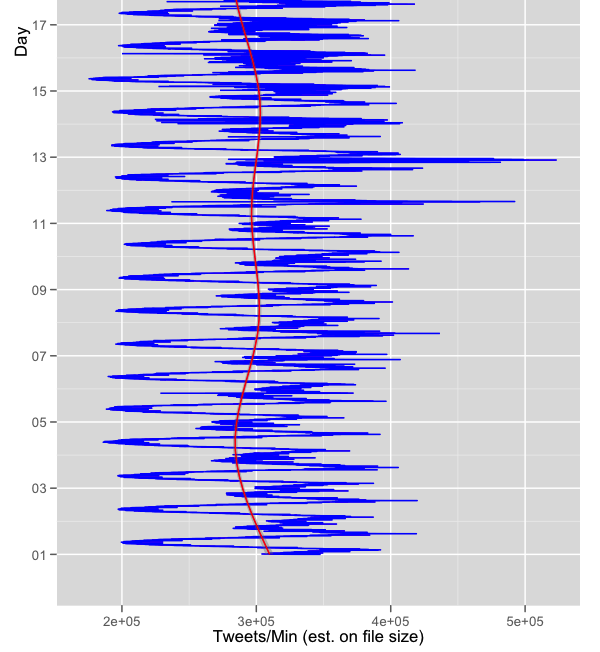
\includegraphics[width=6.5cm]{./imgs/tweets.png}
  \end{center}
\end{frame}

\begin{frame}\frametitle{Twitter volumes - day of week}
  \begin{center}
    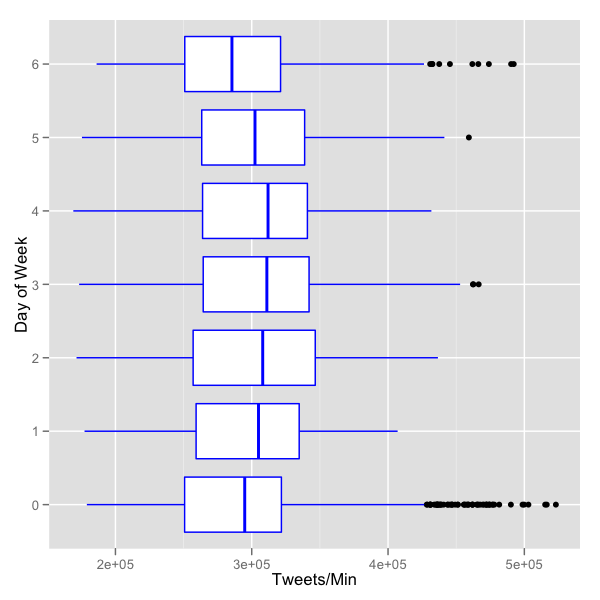
\includegraphics[width=7.5cm]{./imgs/dow.png}
  \end{center}
\end{frame}

\begin{frame}\frametitle{Twitter volumes - hour of day}
  \begin{center}
    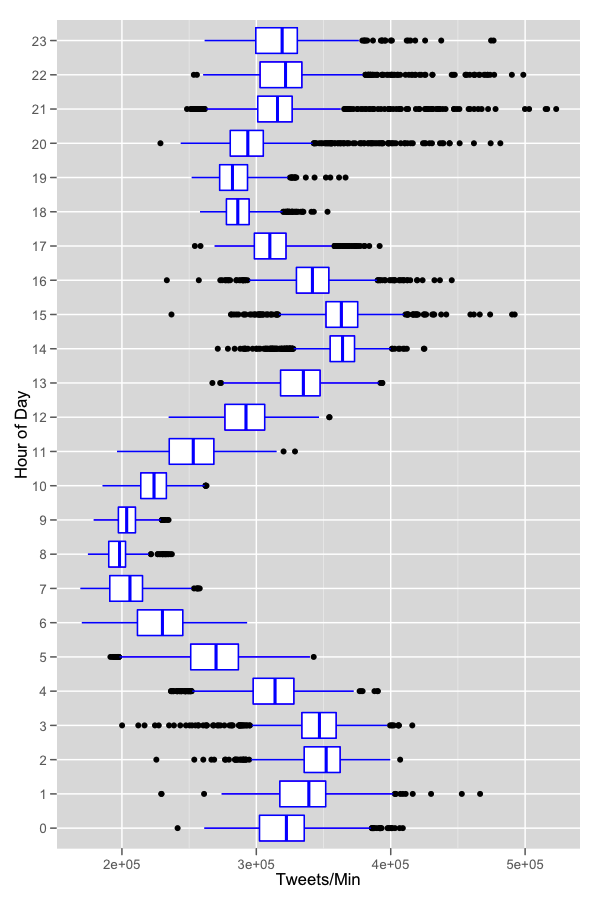
\includegraphics[width=5cm]{./imgs/hour.png}
  \end{center}
\end{frame}

% payload

{
\usebackgroundtemplate{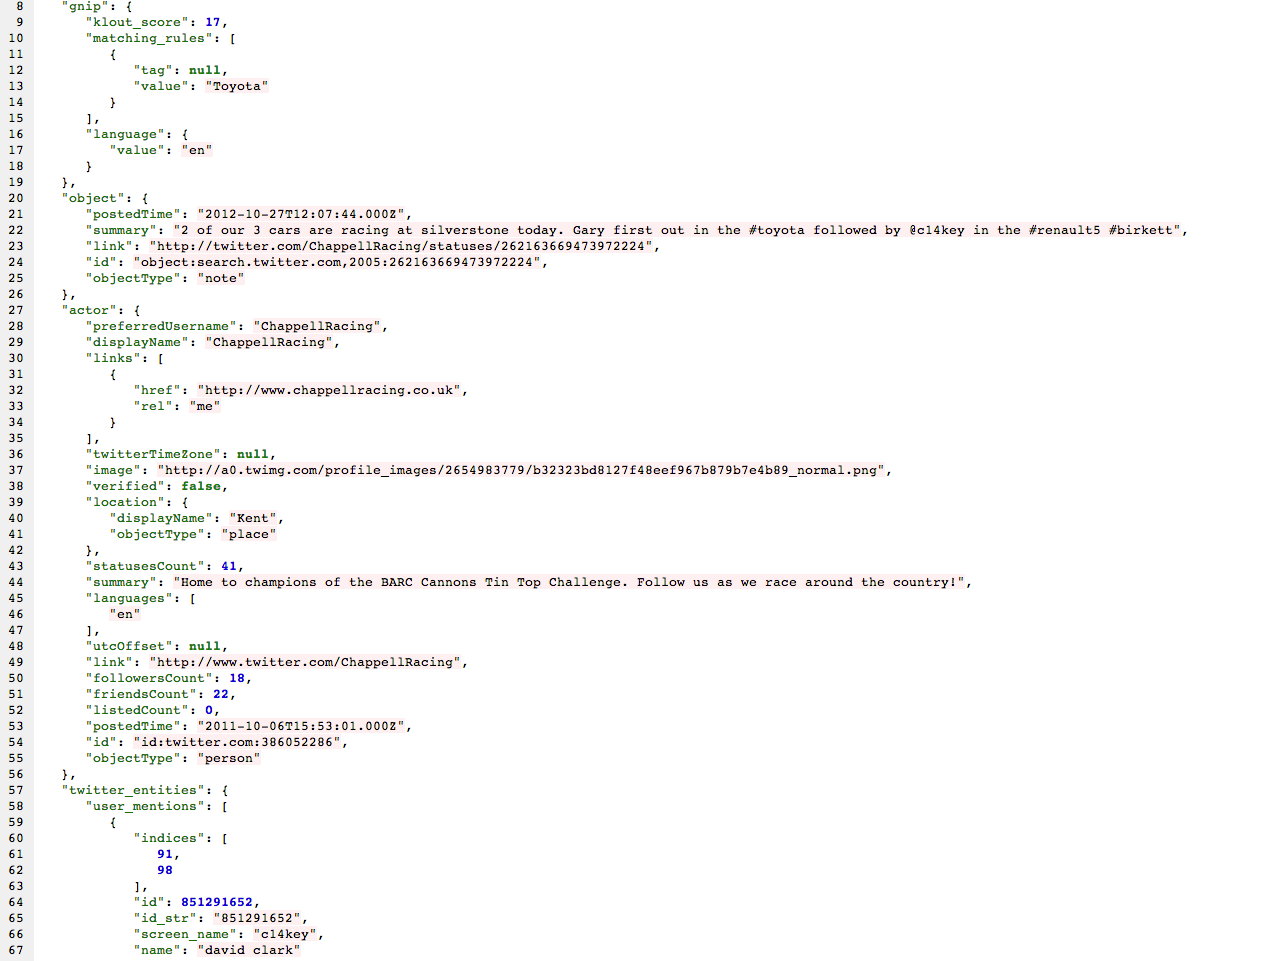
\includegraphics[width=\paperwidth]{./imgs/json.png}}
\begin{frame}\frametitle{\textcolor{black} {Twitter payload}}
  \begin{center}
\textcolor{black} {
\Huge \href{run:./twitter_record.html}{twitter.json} }
  \end{center}
\end{frame}
}

\section{Streaming data from the firehose}

{
\usebackgroundtemplate{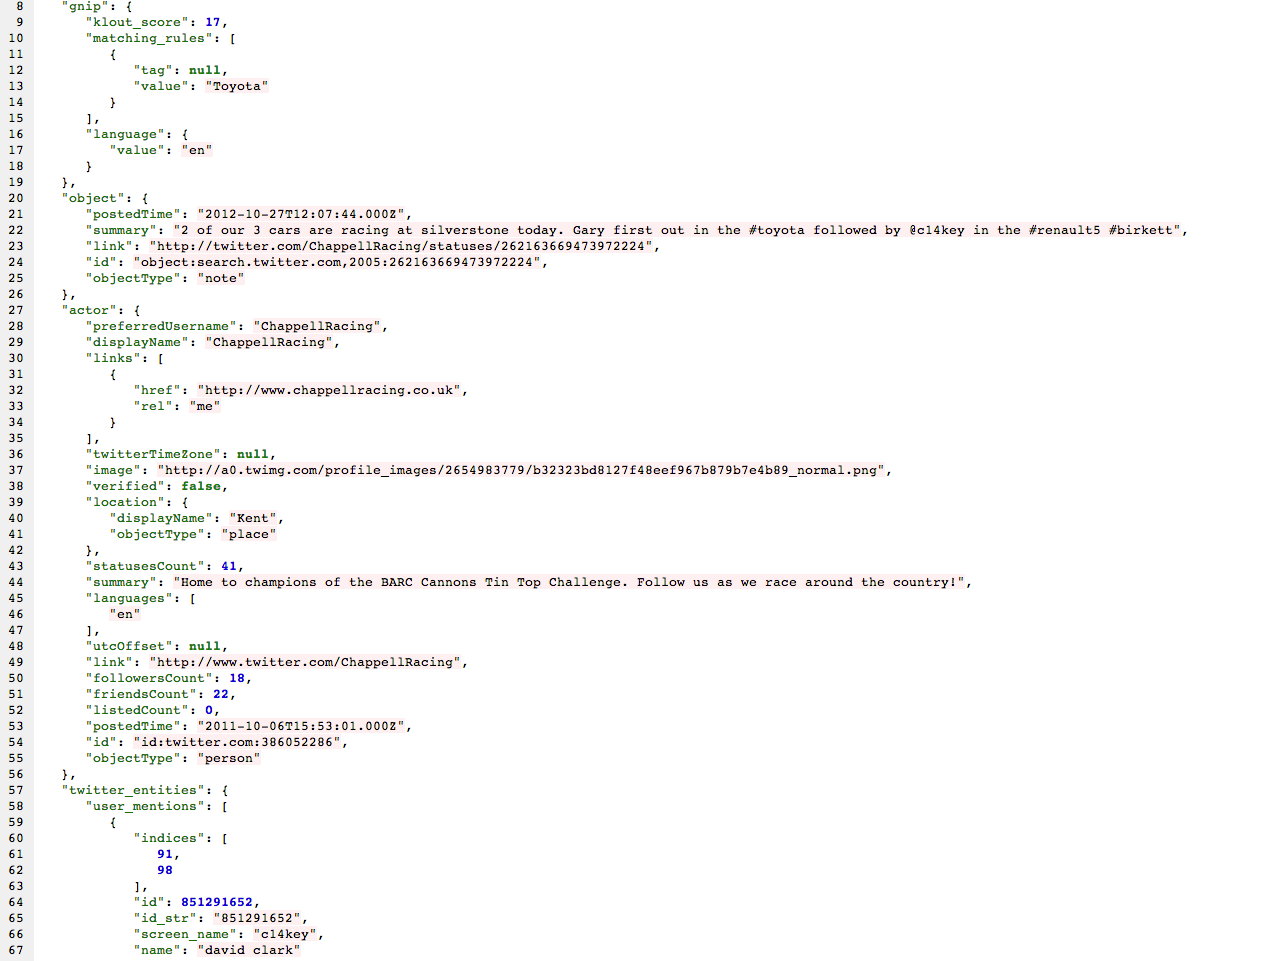
\includegraphics[width=\paperwidth]{./imgs/json.png}}
\begin{frame}\frametitle{\textcolor{black} {Gnip stream management}}
  \begin{center}
\textcolor{black} {
\Huge \href{http://console.gnip.com}{http://console.gnip.com} 
}
  \end{center}
\end{frame}
}

{
\usebackgroundtemplate{\includegraphics[width=\paperwidth]{./imgs/curling.jpg}}
\begin{frame}[fragile]
\Huge{\color{black}\secname{}}
\end{frame}
}

\begin{frame}[fragile]
\frametitle{Curl the firehose}
\begin{verbatim}
curl --compressed -v \
-ushendrickson@gnip.com  \
"https://stream.gnip.com:443/accounts/shendrickson/
     publishers/twitter/streams/track/track2.json"
\end{verbatim}
\end{frame}

\begin{frame}[fragile]
\frametitle{More curling the firehose}
\begin{verbatim}
curl --compressed -s \
-ushendrickson@gnip.com:<password>  \
"https://stream.gnip.com:443/accounts/shendrickson/
    publishers/twitter/streams/track/track2.json" \
-o outfile.json
\end{verbatim}
\end{frame}

\section{PowerTrack}

\begin{frame}\frametitle{PowerTrack: filter and shape}
\begin{itemize}
\item core idea: exact token matches (e.g. "obama", "beer" \ldots)
\item non-token matches: ``happy birthday'' and ``contains:dog''
\item meta-data operators: geo, language, bios, \ldots
\item shaping operators: (e.g. ``sample:10'' gives 10\%)
\item operators: (by publisher) user, hashtag, language,\ldots
\item filter on 100\% of the firehose
\end{itemize}
\end{frame}

% rules combining

\begin{frame}\frametitle{PowerTrack: combining rules}
\begin{equation*}
\begin{aligned}
        newline &= OR \\
        space &= AND \\
        ``OR'' &= OR \\
        ``-'' &= NOT \\
        ``(\ldots)'' &= grouping
\end{aligned}
\end{equation*}
\end{frame}

% limits

\begin{frame}\frametitle{PowerTrack: rule limits}
\begin{itemize}
\item A single PowerTrack rule may contain up to 10 positive clauses, and up to 50 negative clauses
\item A single PowerTrack rule may not have more than 1024 characters, including OR operators and parentheses
\item Max 250K rules
\end{itemize}
\end{frame}

% rules examples

\begin{frame}[fragile]\frametitle{Example Toyota PowerTrack rules}
\begin{verbatim}
(sexy OR speed OR speeding OR \"sport utility\" OR ...
    suv OR toyota) (infiniti OR infinitis OR #infiniti OR @infiniti) -job 
    -\"<money>\" -\"<phone>\" -jobs -deal -review -#jobs -tattoo
    -giveaway -deals -discount -reviews -#job -jewelry -jewelry
@toyotacanada sample:40
lang:en toyota recall
lang:it toyota window
lang:fr toyota recall
lang:en toyota auris -crime -lease -sells -thief -police -robbed -robber
lang:ru toyota dyna -lkw -aqua -bail -died -film -toka -camry
\end{verbatim}
\end{frame}

\begin{frame}\frametitle{Enterprise PowerTrack features}
\begin{itemize}
\item Update individual rules without disconnect ( $\lesssim1s$ update time for 100s of rules)
\item Rule tagging
\item Keep alive - signal that connection is live, even when no data is coming (30 s)
\item Low latency: avg 1s Twitter raw; 10s Twitter enriched
\item Redundancy - multiple simultaneous connections available
\item Backfill - buffer data and fill in if short term disconnect
\item PowerTrack Replay - connect with start and end dates to stream past time periods (<5 days)
\item Historical PowerTrack - Twitter historical filtering for any time period
\end{itemize}
\end{frame}

% rules API

\begin{frame}[fragile]\frametitle{Rule JSON}
\begin{verbatim}
{
   "rules": [
      {
         "tag": "presidents", 
         "value": "obama"
      }, 
      {
         "tag": "musicians", 
         "value": "gaga"
      }, 
      {
         "tag": "musicians", 
         "value": "bieber"
      }
   ]
} 
\end{verbatim}
\end{frame}

\begin{frame}\frametitle{Rules REST API}
\begin{itemize}
\item POST (add rules)
\item DELETE (rule match by value)
\item GET (rule list)
\item UPDATE pattern: GET, (alter rule), ADD, DELETE
\item https://api.gnip.com:443/accounts/shendrickson/\\
    publishers/twitter/streams/track/track2/rules.json
\end{itemize}
\end{frame}

{
\usebackgroundtemplate{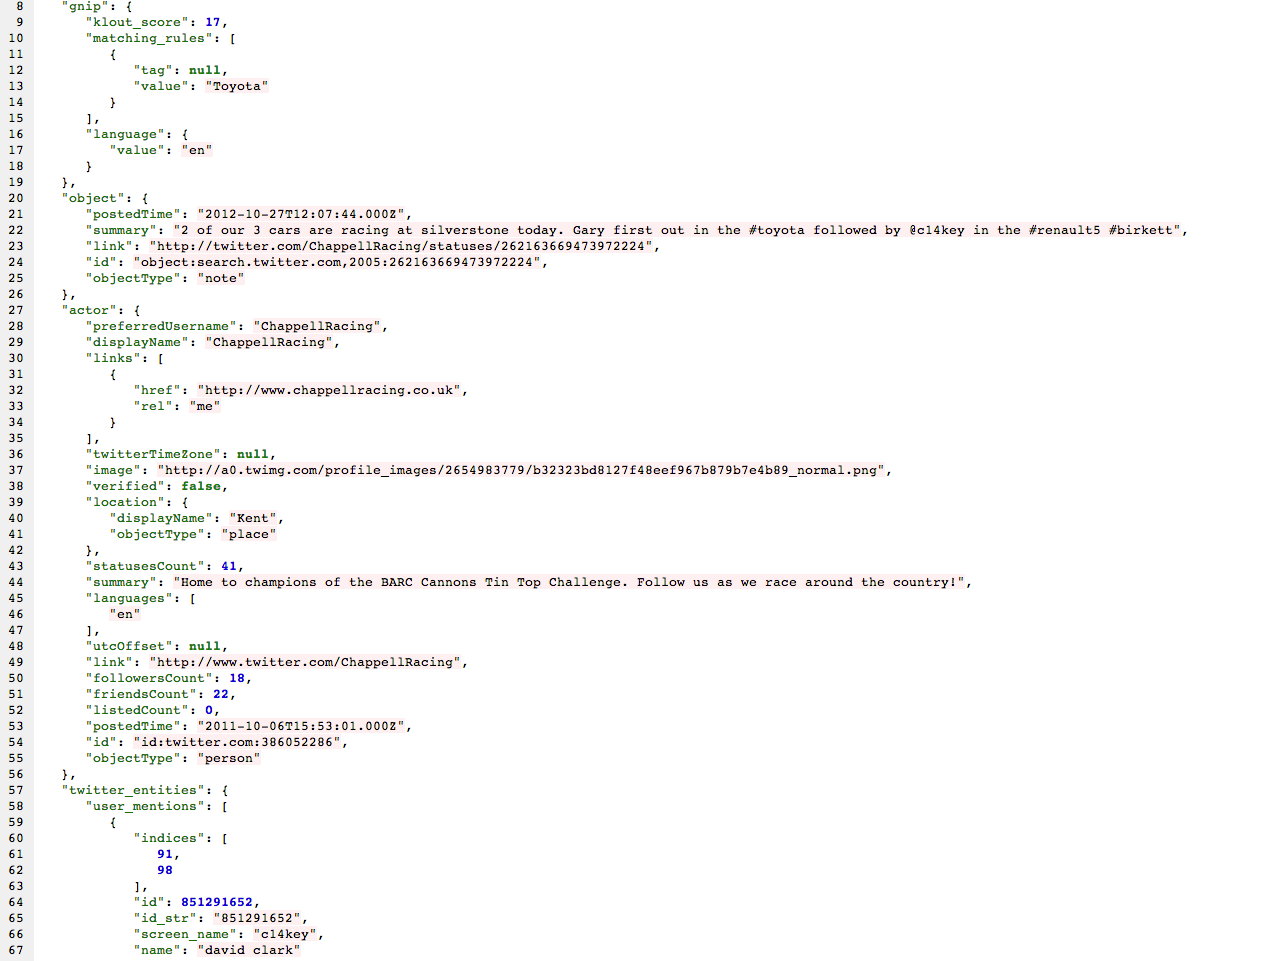
\includegraphics[width=\paperwidth]{./imgs/json.png}}
\begin{frame}\frametitle{\textcolor{black} {Twitter PowerTrack documentation}}
  \begin{center}
\textcolor{black} {
\Large \href{http://docs.gnip.com/}{http://docs.gnip.com} \\ [20 pt]
\href{http://support.gnip.com/customer/portal/articles/901152-powertrack-operators}{http://support.gnip.com/customer/portal/ articles/901152-powertrack-operators} }
  \end{center}
\end{frame}
}

\section{Tools}
{
\usebackgroundtemplate{\includegraphics[width=\paperwidth]{./imgs/curling.jpg}}
\begin{frame}[fragile]
\Huge{\color{black}\secname{}}
\end{frame}
}

\begin{frame}\frametitle{Simple parser: TWitterACTivitieS}
\begin{itemize}
\item core idea: use twacs to parse common twitter elements to pipe-delimited (flat) structure
\item requires: Python
\item github: https://github.com/DrSkippy27/Twacs
\item From PyPi: sudo pip install twacs 
\end{itemize}
\end{frame}

\begin{frame}[fragile]
\frametitle{twacs.py examples - prettifier}
\begin{verbatim}
> gzip -cd twitter_oneDay_onePercent.json.gz | twacs-prettifier.py 
{
   "body": "Giving them 1 inch and they take a mile", 
   "retweetCount": 0, 
   "generator": {
      "link": "http://twitter.com/download/iphone", 
      "displayName": "Twitter for iPhone"
   }, 
   "gnip": {
      "klout_score": 47, 
      "language": {
         "value": "en"
      }
   }, 
\end{verbatim}
\ldots
\end{frame}

\begin{frame}[fragile]
\frametitle{twacs.py examples - basic parse}
\begin{verbatim}
> gzip -cd twitter_oneDay_onePercent.json.gz | twacs.py 
tag:search.twitter.com,2005:309063808016584704|
      2013-03-05T22:12:08.000Z|
      Giving them 1 inch and they take a mile
tag:search.twitter.com,2005:309063808041771008|
      2013-03-05T22:12:08.000Z|
      @luizaaguiarb só se for o teu filho! O meu vai ser super higienizado e cheiroso! Sai!
tag:search.twitter.com,2005:309063808331153409|
      2013-03-05T22:12:08.000Z|
      @SlyOuu Mdrrr le negro s'emballe les coquilles
tag:search.twitter.com,2005:309063808427622402|
      2013-03-05T22:12:08.000Z|
      RT @NotARapistHere: My favorite pickup line: Get in the van.
 Audsbgivasiugbasdpiub
\end{verbatim}
\ldots
\end{frame}

\begin{frame}[fragile]
\frametitle{twacs.py examples - help}
\begin{verbatim}
>twacs.py -h
Usage: twacs.py [options]

Options:
  -h, --help       show this help message and exit
  -g, --geo        Include geo fields
  -u, --user       Include user fields
  -r, --rules      Include rules fields
  -s, --urls       Include urls fields
  -l, --lang       Include language fields
  -p, --pretty     Pretty JSON output of full records
  -c, --csv        Comma-delimited output (default is | without quotes)
  -x, --explain    Show field names in output for for sample input records
  -i, --influence  Show user's influence metrics
\end{verbatim}
\end{frame}


\begin{frame}[fragile]
\frametitle{Curling and parsing the firehose}
\begin{verbatim}
curl --compressed -s \
-ushendrickson@gnip.com:<password>  \
"https://stream.gnip.com:443/accounts/shendrickson/
     publishers/twitter/streams/track/track2.json" | twacs.py
\end{verbatim}
\end{frame}

% powertrack rules

\begin{frame}\frametitle{Rules management}
\begin{itemize}
\item core idea: use to list, delete, add  and update rules
\item requires: Python
\item library and command line utilities
\item github: https://github.com/DrSkippy27/Gnip-Python-PowerTrack-Rules
\end{itemize}
\end{frame}

{
\usebackgroundtemplate{\includegraphics[width=\paperwidth]{./imgs/curling.jpg}}
\begin{frame}[fragile]
\Huge{\color{black}Twitter stream \\ [10pt] attributes}
\end{frame}
}

\section{Replies and retweets}

\begin{frame}[fragile]
\frametitle{inReplyTo data element}
\begin{verbatim}
{
   "body": "@rachelschadd @kylefraley3 @toritabin don't read, just tweet!", 
   "inReplyTo": {
      "link": "http://twitter.com/rachelschadd/statuses/309064691186020352"
   }

{
   "body": "@stonesy10 clearly but Madrid can!! Arsenal won't have to 
          worry bout that next season though", 
   "inReplyTo": {
      "link": "http://twitter.com/stonesy10/statuses/309063725309104128"
   }
\end{verbatim}
\end{frame}



\begin{frame}[fragile]\frametitle{Retweets}
\begin{itemize}
\item about 17\% of twitter activities are retweets
\item convention ``RT \ldots'' added by many clients to text
\item unattributed quoting
\end{itemize}
\begin{verbatim}
{
   "body": "RT @UberBulIshit: Snoop Dogg changed his name to Snoop 
             Lion after losing a bet in which he was out-smoked by Justin Bieber.", 
   "retweetCount": 1979, 
...
\end{verbatim}
\end{frame}


\begin{frame}[fragile]\frametitle{Retweets link}
\begin{verbatim}
      "object": {
         "postedTime": "2013-03-05T22:08:54.000Z", 
         "summary": "Fergie, that was for Jonjo Shelvey.", 
         "link": "http://twitter.com/KopiteKru/statuses/309062995366010882"
...
\end{verbatim}
\href{http://twitter.com/KopiteKru/statuses/309062995366010882}{http://twitter.com/KopiteKru/statuses/309062995366010882}
\end{frame}         
         
\section{Languages}

% twitter lang 1

\begin{frame}\frametitle{Twitter bio langauges}
  \begin{center}
    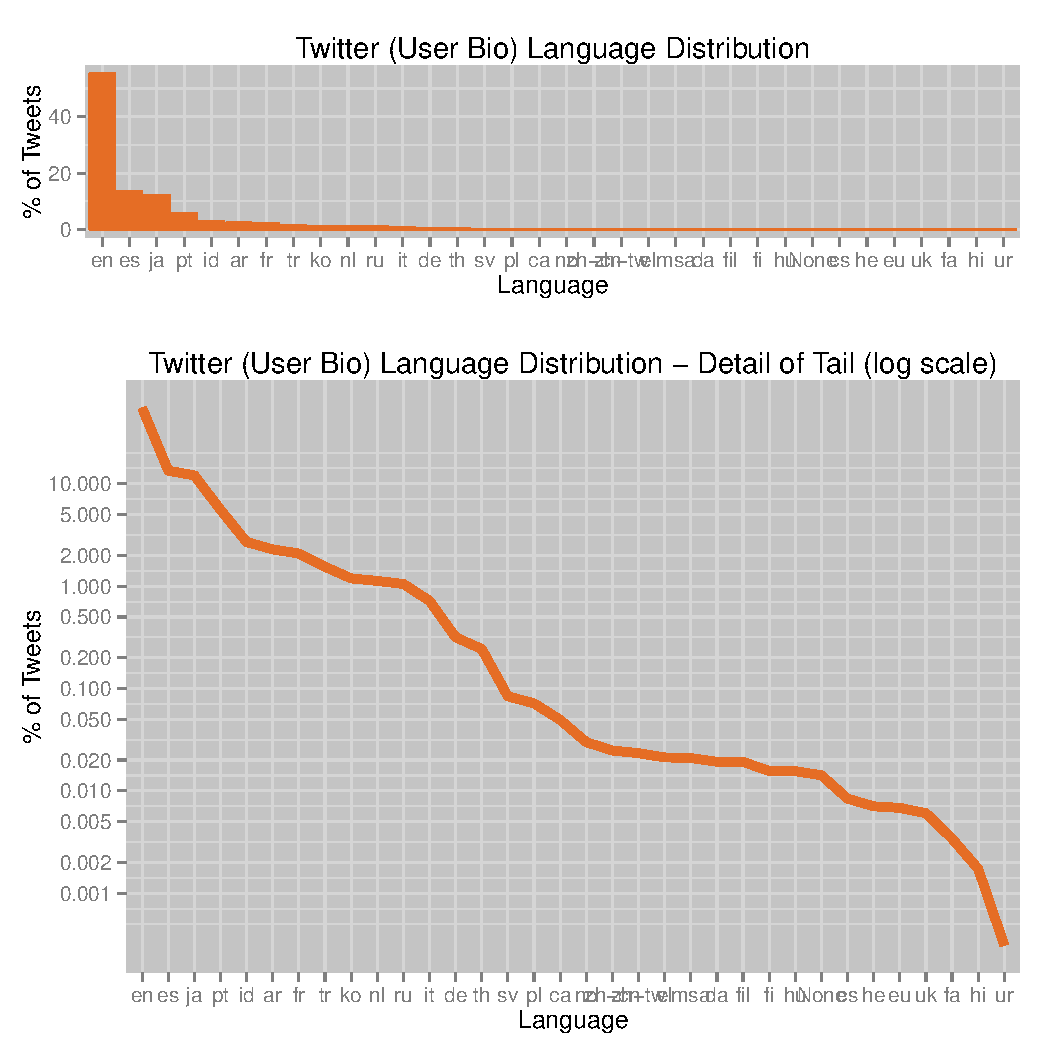
\includegraphics[width=7.5cm]{./imgs/distro_bio.pdf}
  \end{center}
\end{frame}

% twitter lang 1

\begin{frame}\frametitle{Twitter tweet (Gnip) languages}
  \begin{center}
    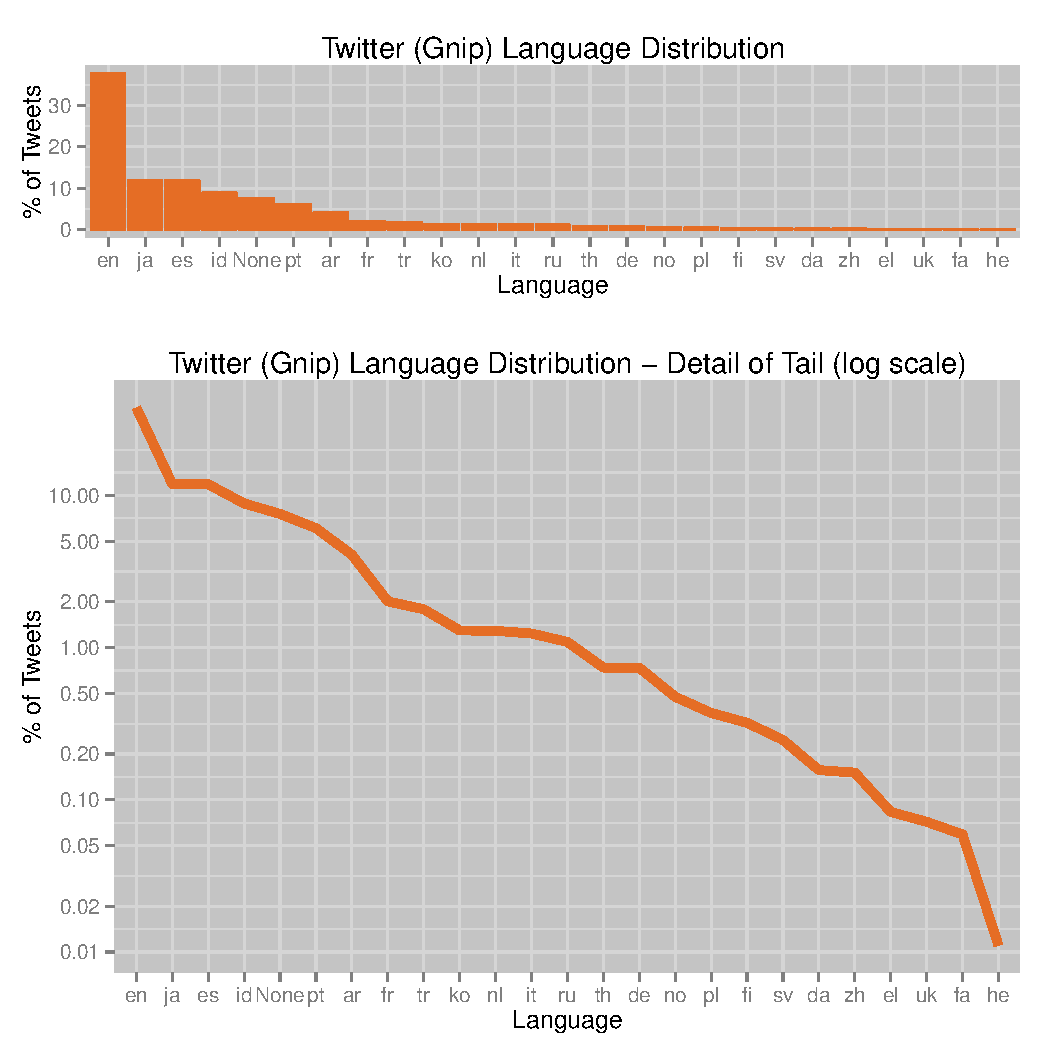
\includegraphics[width=7.5cm]{./imgs/distro_gnip.pdf}
  \end{center}
\end{frame}

% twitter lang 1

\begin{frame}\frametitle{Twitter bio vs. tweet languages}
  \begin{center}
    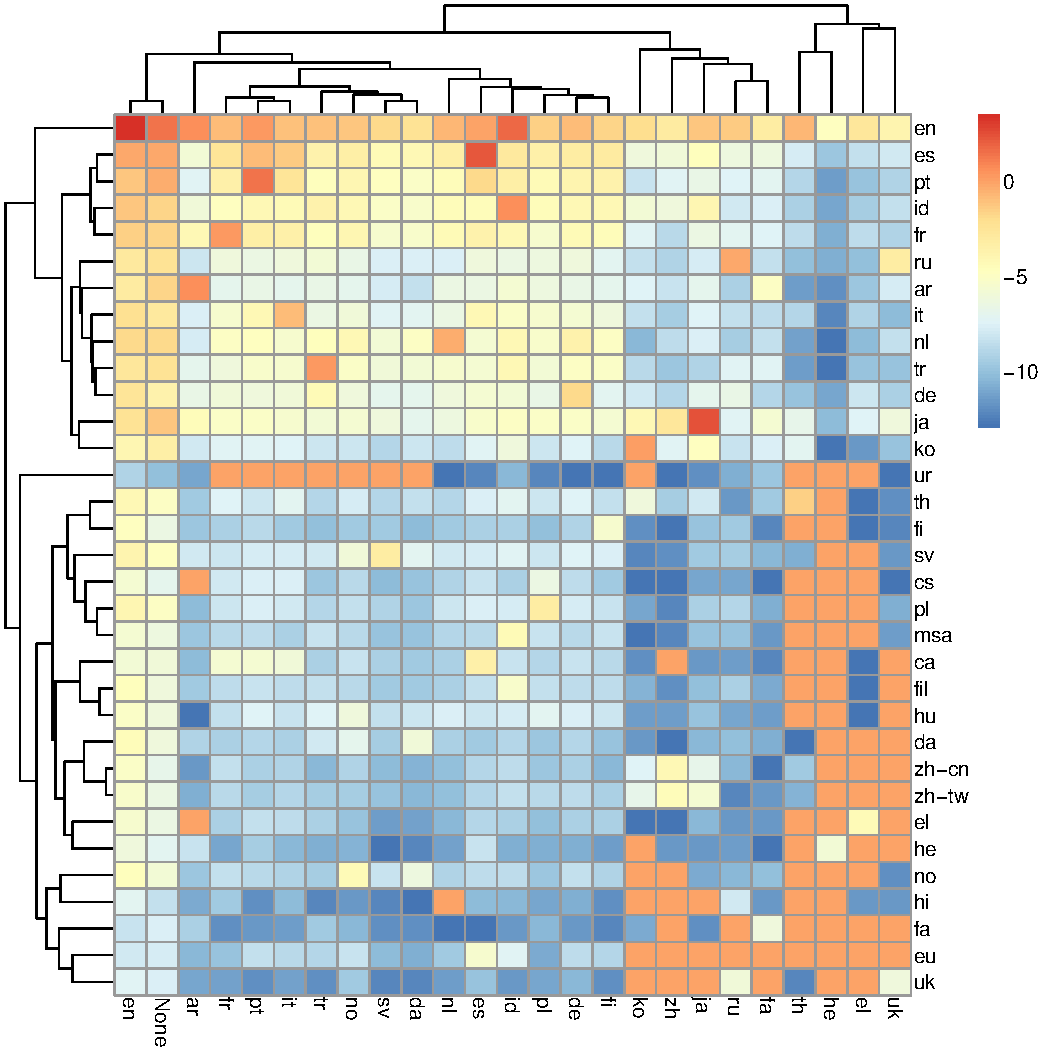
\includegraphics[width=7.5cm]{./imgs/heatmap.pdf}
  \end{center}
\end{frame}


\section{Geolocation}


\begin{frame}[fragile]
\frametitle{Geo information in tweets}
\begin{verbatim}
[ tweet location] | Tweet location place id'd by twitter | User bio location
--------------------------------------------------------------------------------------
['41.02117698', '-73.8731331']|Mercy College, Dobbs Ferry|US|NYC
['-7.54556', '110.82484']|Banjarsari, Surakarta|ID|Indonesia
['51.7541896', '-0.34086304']|Saint Albans, Hertfordshire|GB|St Albans
['51.8446547', '4.3364468']|Spijkenisse|NL|DEDICATED FOR LIFE
['18.22484423', '-65.9027102']|Ceiba Norte, PR|US|Juncos
['40.21630994', '28.96884114']|Türkiye|TR|Erdek /Bursa
['36.89167243', '30.67495879']|Türkiye|TR|big drummer
['-6.2590775', '106.868624']|Kramat Jati, Jakarta Timur|ID|Random
\end{verbatim}
\end{frame}

\begin{frame}\frametitle{Geo location of Tweets}
\begin{table}
\begin{tabular}{ m{3.5cm} | m{3cm} | m{2cm}}
\hline
Type & Precision & Frequency \\ \hline
Geo Tagged: (Lat, Long) "Point"	& High & 1.235\% \\ \hline
 Geo Tagged: (Lat, Long) points "Polygon" & Medium-Low	& 1.418\% \\ \hline
 -- & With either Point, Polygon or Both & 1.596\% \\\hline
 Country Code &	Medium & 1.43\% \\ \hline
 User Bio Place & High (long, lat)-Low (gibberish) &57.67\% \\ \hline
 Timezone Offset & Medium-Low & 73.6\% \\
 \hline
\end{tabular}
\end{table}
\end{frame}

% social media pulse

\section{Social media pulse}

{
\usebackgroundtemplate{\includegraphics[width=\paperwidth]{./imgs/curling.jpg}}
\begin{frame}[fragile]
\Huge{\color{black}\secname{}}
\end{frame}
}

% staging the question

\begin{frame}
\begin{center}
{\Huge Audience \& perspective, Timing}
\end{center}
\end{frame}

% toyota
\begin{frame}
  \begin{center}
    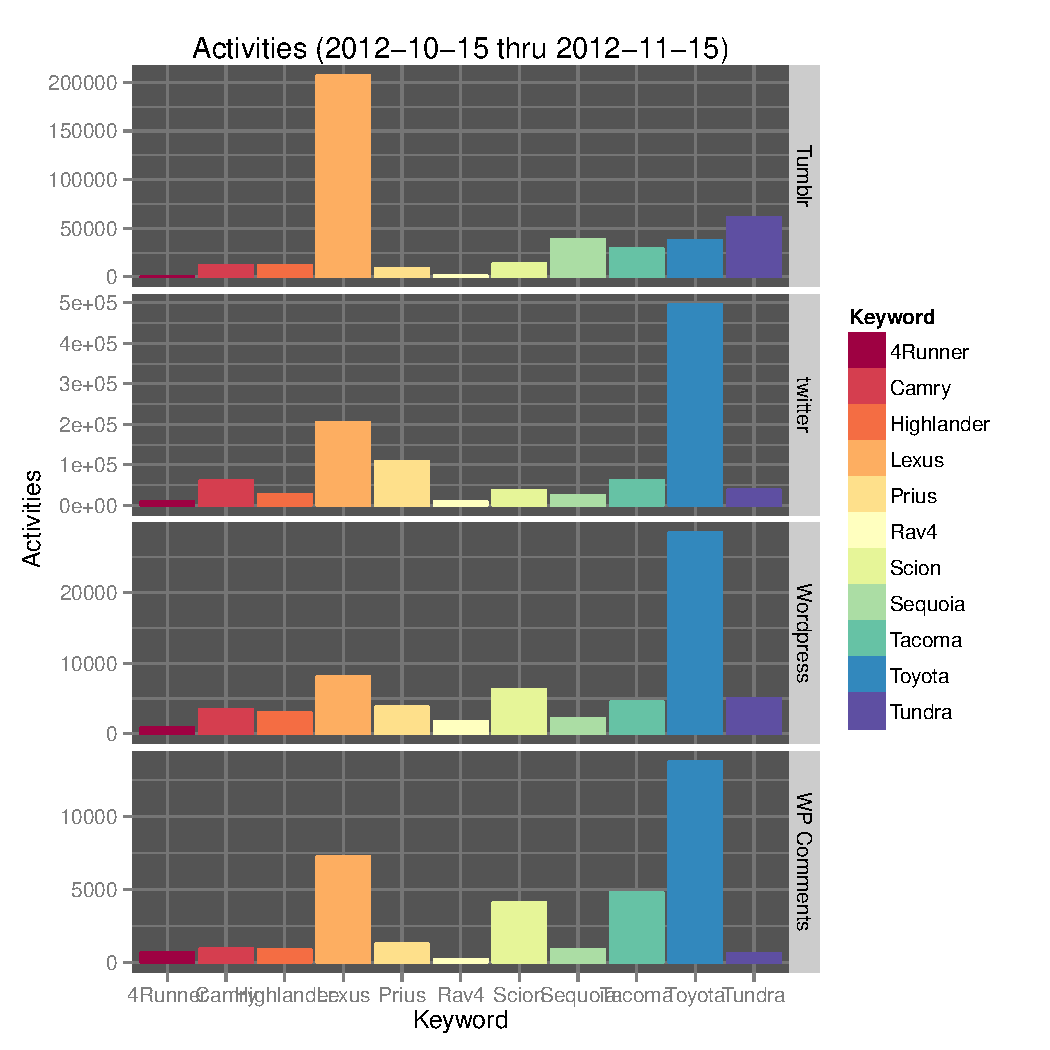
\includegraphics[width=8cm]{./imgs/bars.pdf}
  \end{center}
\end{frame}

% signal vs. noise

\begin{frame}
\begin{center}
\center{\Huge {noise or signal?}}
\end{center}
\end{frame}

% chelsea con-ed example

\begin{frame}\frametitle{Sandy -- Chelsea Power Outage}
  \begin{center}
    \includegraphics[width=8cm]{./imgs/fake.pdf}
  \end{center}
\end{frame}


\begin{frame}\frametitle{Better Statistical Model}
  \begin{center}
    \includegraphics[width=8cm]{./imgs/fake_fit2.pdf}
  \end{center}
\end{frame}

\begin{frame}\frametitle{Real event has much higher volume}
  \begin{center}
    \includegraphics[width=8cm]{./imgs/real_fit.pdf}
  \end{center}
\end{frame}


\begin{frame}\frametitle{Expected: Hurricane}
  \begin{center}
    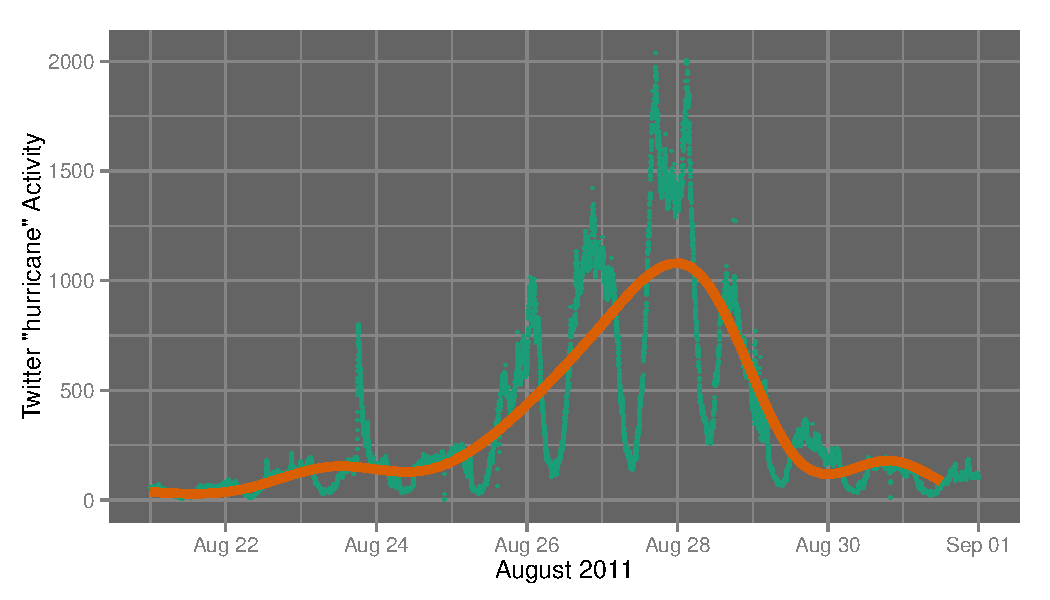
\includegraphics[width=11cm]{./imgs/hurricane_trend.pdf}
  \end{center}
\end{frame}
%
%\begin{frame}\frametitle{Unexpected: Earthquake}
%  \begin{center}
%    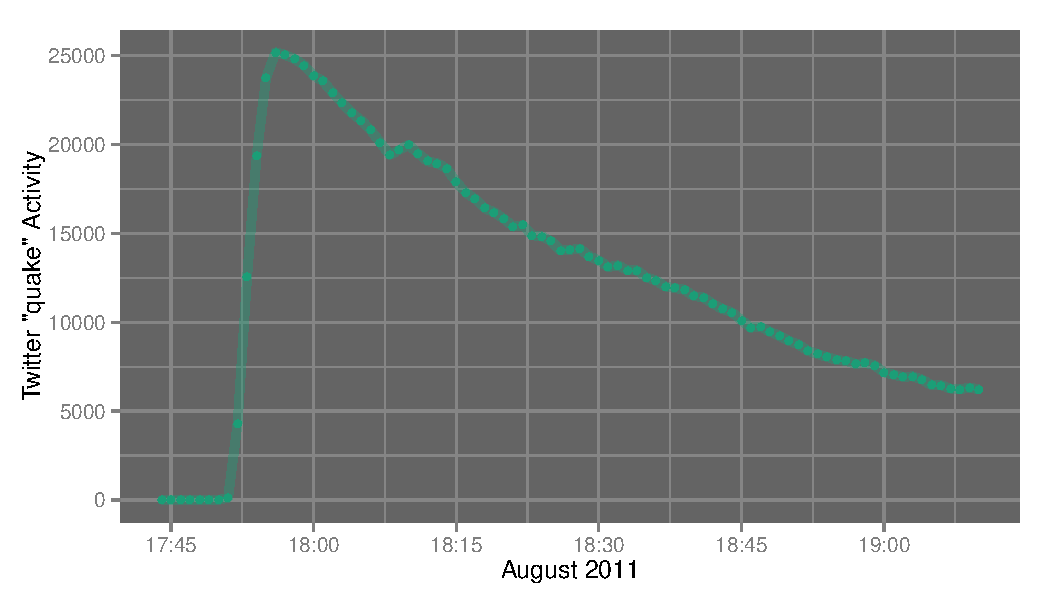
\includegraphics[width=11cm]{./imgs/va_quake.pdf}
%  \end{center}
%\end{frame}

\begin{frame}\frametitle{Unexpected: Earthquake}
  \begin{center}
    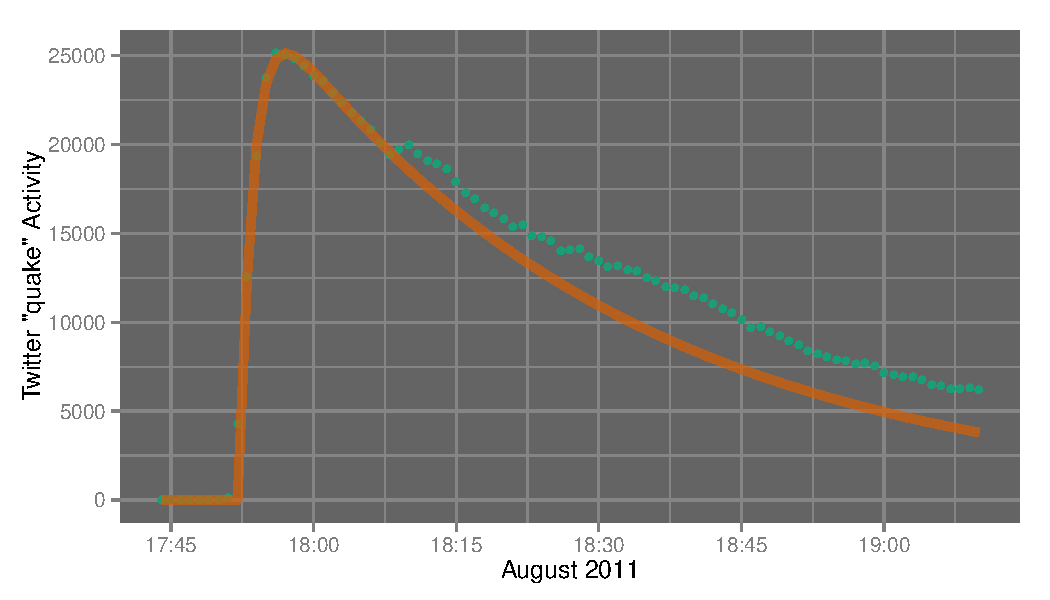
\includegraphics[width=11cm]{./imgs/va_quake_fit1.pdf}
  \end{center}
\end{frame}

% Events

\begin{frame}\frametitle{Classifying Events}
\begin{table}
\begin{tabular}{ m{2cm} | m{ 2.5cm} | m{4cm}}
\hline
Type & Response & Examples \\ \hline
Expected    & Approx. \newline Symmetric & Hurricane Sandy \newline Olympics \\ \hline
Unexpected (many obs.) & Social Media \newline Pulse & Beyonc\'{e} VMAs \newline  Mexico earthquake \newline  Steve Jobs \\ \hline
Unexpected (spread) & Network \newline Models & Osama bin Laden \newline  Whitney Houston \newline  Syrian dissidents \\ \hline
\end{tabular}
\end{table}
\end{frame}


% half life

\begin{frame}\frametitle{Half-life}
\begin{center}
{\Huge time to observe \\[6pt] $\frac{1}{2}$ of the activities \\[6pt] for an event}
\end{center}
\end{frame}

\begin{frame}
\frametitle{Social media pulse} 
Given an event, the probability of a activity from one person,

\begin{equation*}
f(t) = \lambda \exp(-\lambda t), \text{ for } t \geq 0.
\end{equation*}

Many people posting, so sum of random variables $S = X_1 + X_2 + \ldots + X_{n \text{ posters}}$.

Probability distribution function,

\begin{equation*}
f_S(t) = \frac{ \beta^{-\alpha} t^{\alpha-1} \exp( \frac{-t}{\beta}) } {\Gamma(\alpha)}
\end{equation*}

Cumulative distribution is the ``generalized regularized incomplete gamma function'',

\begin{equation*}
F_S(t) = Q(\alpha, 0, \frac{ t}{\beta})
\end{equation*}
\end{frame}

% gamma plots

\begin{frame}
  \begin{center}
   \includegraphics[height=6cm]{./imgs/gammadist.pdf}
  \end{center}
\end{frame}
\begin{frame}\frametitle{Why model half-life?}
\begin{center}
\begin{itemize}
\Huge{
\item predict total story volume
\item compare half-lives
\item anomalous story evolution
}
\end{itemize}
\end{center}
\end{frame}


\begin{frame}
  \begin{center}
    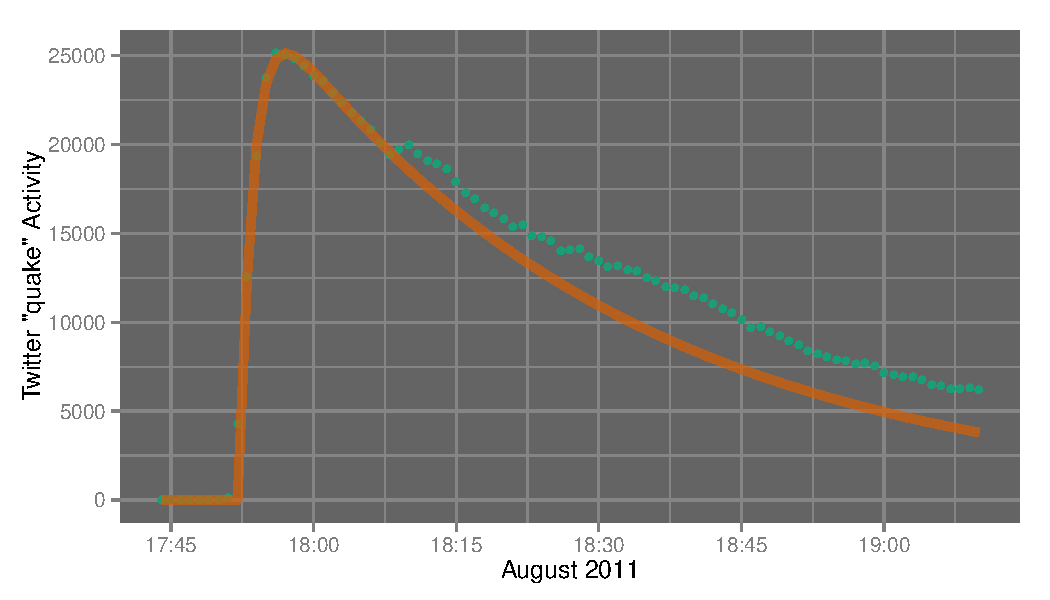
\includegraphics[width=8cm]{./imgs/va_quake_fit1.pdf}
  \end{center}
\end{frame}



% JPMorgan

\begin{frame}
  \begin{center}
    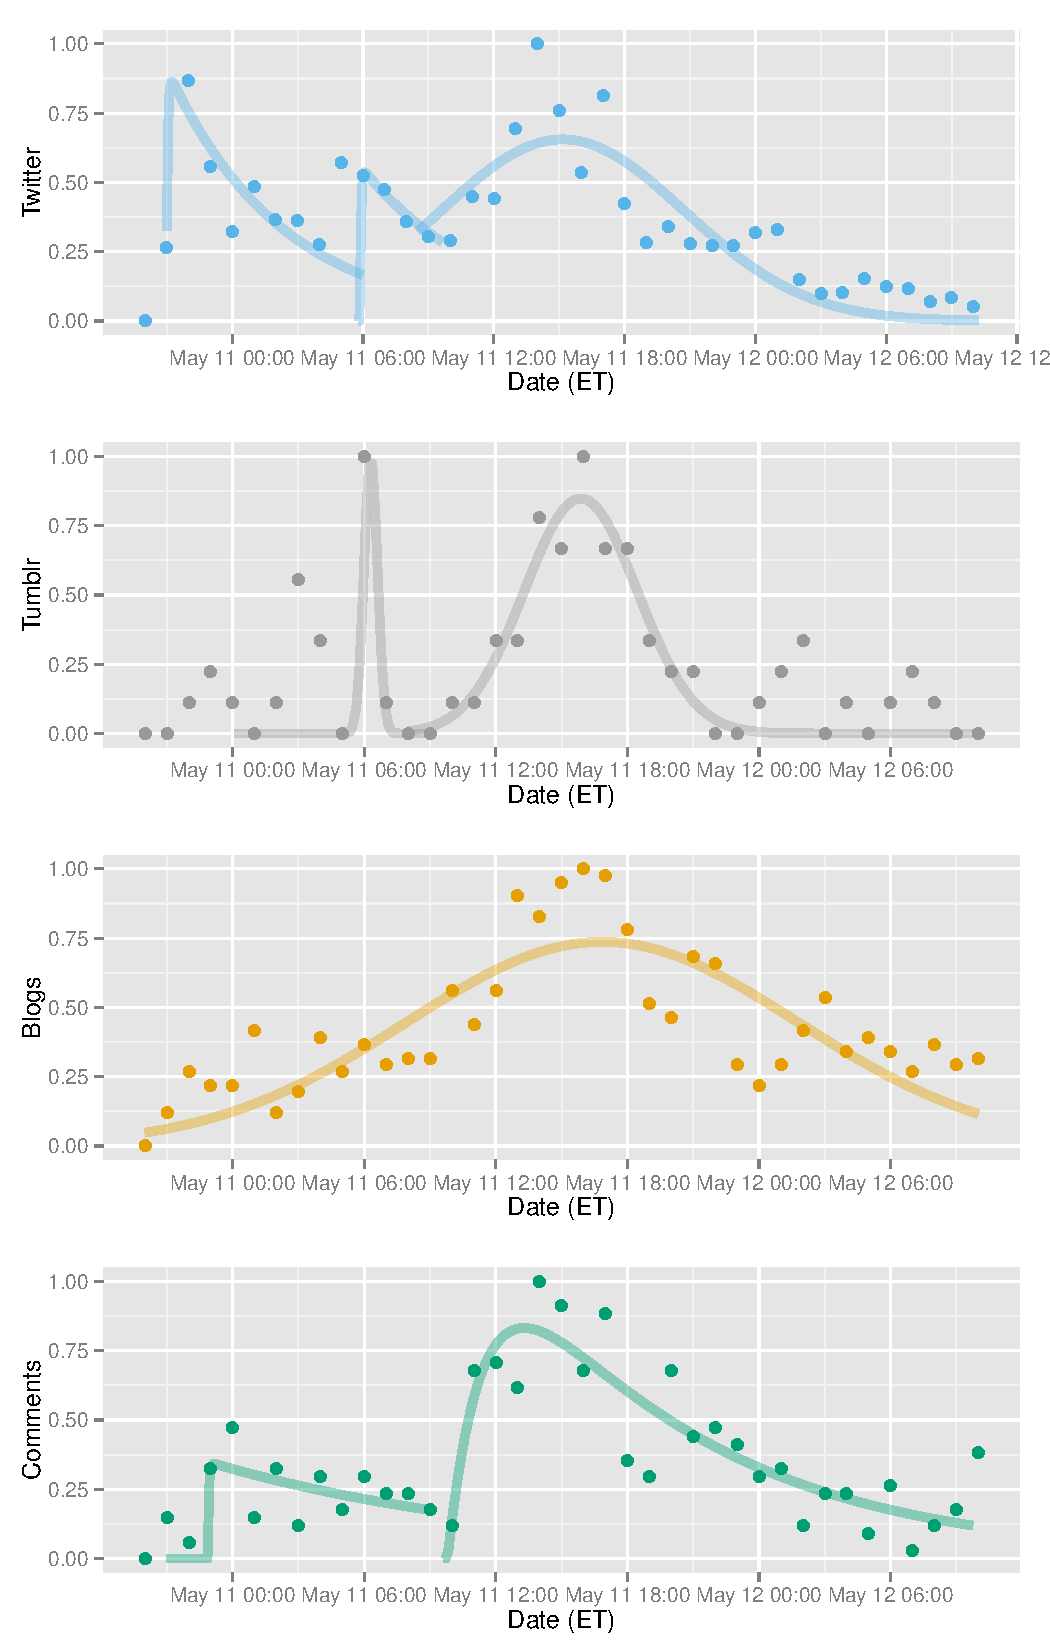
\includegraphics[height=8.5cm]{./imgs/JPMorgan.pdf}
  \end{center}
\end{frame}

% the end

\begin{frame}
  \begin{center}
    {\Large Thank you!}  \\ [20pt]
    \includegraphics[width=3cm]{./imgs/logo.png} \\ [15pt]
    \begin{itemize}
    \item Presentation, data, code at: \url{http://github.com/DrSkippy27/GreenPlum2013}
    \end{itemize}
  \end{center}
\end{frame}

\end{document}
